\documentclass{beamer}
\usepackage{../../shared/styles/custom}
\usepackage{../../shared/styles/conventions}

%\beamerdefaultoverlayspecification{<+->}
% \newcommand{\data}{\mathcal{D}}
% \newcommand\Item[1][]{%
% 	\ifx\relax#1\relax  \item \else \item[#1] \fi
% 	\abovedisplayskip=0pt\abovedisplayshortskip=0pt~\vspace*{-\baselineskip}}

\graphicspath{ {../assets/bias-variance/figures/} }

\title{Bias-Variance}
\date{\today}
\author{Nipun Batra and teaching staff}
\institute{IIT Gandhinagar}
\begin{document}
	\maketitle

\begin{frame}Here, the true function $f_{\vtheta_{\text{true}}}$ is used to model the relation $y_t = f_{\vtheta_{\text{true}}}(x_t)$
\begin{figure}
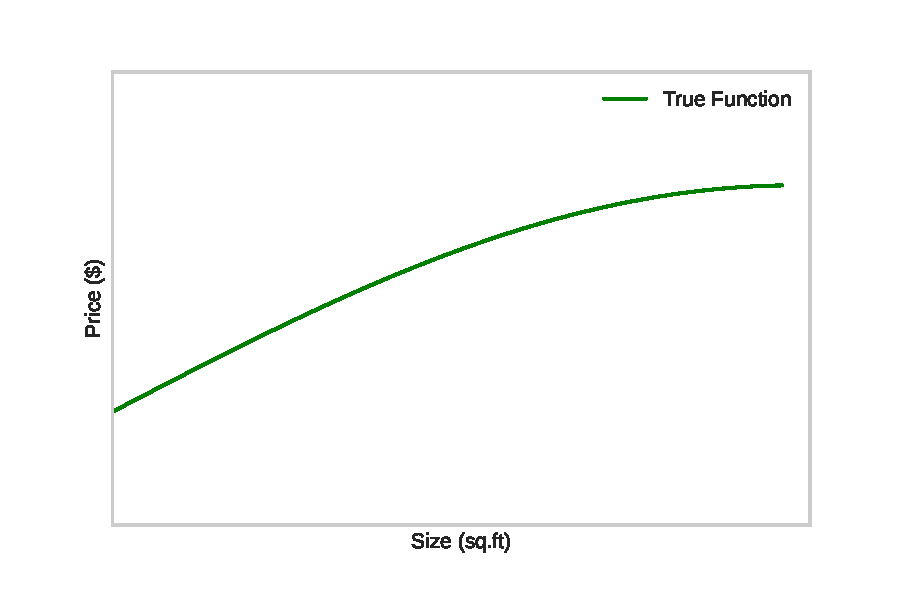
\includegraphics[width=0.6\textwidth]{../assets/bias-variance/figures/true.pdf}
\vspace*{-0.3cm}
\caption{Modeling the relation}
\end{figure}
\end{frame}

\begin{frame}This behavior varies due to training set randomness.
\pause 

Therefore, it is important to measure performance \textbf{averaged over all possible training sets} (of size N). 
\pause

$$E_{\text{training set}}[\text{error of } \hat\theta(\text{training set})] $$
gives a measure of the average error by doing an expectation of the errors of all possible training sets of size N.
\end{frame}

\begin{frame}Therefore, $E_{train}[\text{at a point } x_t] = f(\text{noise, bias, variance}) $ 

\end{frame}

\begin{frame}{Formally defining the 3 sources of error: Noise}
\only<1->{Noise is an \textbf{irreducible error} captured by the error term $\epsilon$.

The equation of the relation becomes $y_t = f_{\theta (true)}(x_t)+\epsilon_t$}

\only<2->{The noise is mean-centered around $0$ with spread called the variance of the noise, denoted by $\sigma^2$. }

\only<3>{That is, it can be denoted by $\epsilon_t \sim \cN(0, \sigma^2)$}

\vspace*{-0.6cm}
\only<2>{\begin{figure}
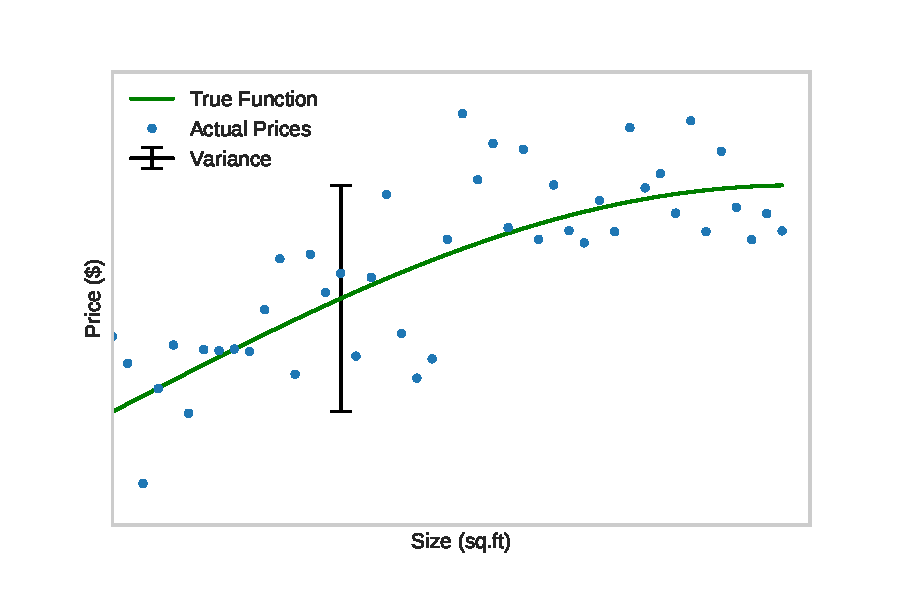
\includegraphics[width=0.7\textwidth]{../assets/bias-variance/figures/data_var.pdf}
\vspace*{-0.3cm}
\caption{Variance in the noise}
\end{figure}}

\end{frame}

\begin{frame}{Formally defining the 3 sources of error: Bias}
\only<1->{Bias is a measure of how flexible the fit is in capturing the true function $f_{\vtheta_{\text{true}}}(x)$}
\only<1->{$$\text{Bias}(x_t) = f_{\vtheta_{\text{true}}}(x_t) - f_{\bar{\vtheta}}(x_t)$$
where $f_{\bar{\vtheta}}$ denotes the average fit over all datasets.
}
\only<1>{\begin{figure}
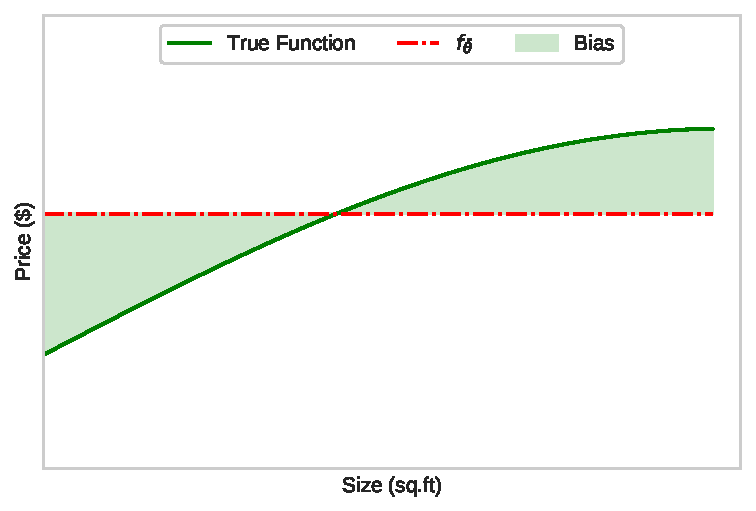
\includegraphics[width=0.65\textwidth]{../assets/bias-variance/figures/bias6.pdf}
\vspace*{-0.3cm}
\caption{Bias of the fit}
\end{figure}}

\only<2->{As $f_{\bar{\vtheta}}$ denotes the average fit over all datasets, it can be expressed by $f_{\bar{\vtheta}}(x_t) = E_{\text{train}}[f_{\hat{\vtheta}}(x_t)]$
}
\end{frame}

\begin{frame}{Formally defining the 3 sources of error: Variance}
\only<1->{Variance of the fit is a measure of the variation in the fits when trained across different training sets.}

\only<2->{Variance of the fit can be defined by
$$\text{var}(f_{\hat{\vtheta}}(x_t)) = E_{\text{train}}[(f_{\hat{\vtheta}}(x) - f_{\bar{\vtheta}}(x_t))^2]$$

where $f_{\hat{\vtheta}}(x) - f_{\bar{\vtheta}}(x_t)$ denotes the deviation that a specific fit has from the average.
}
\only<1>{\begin{figure}
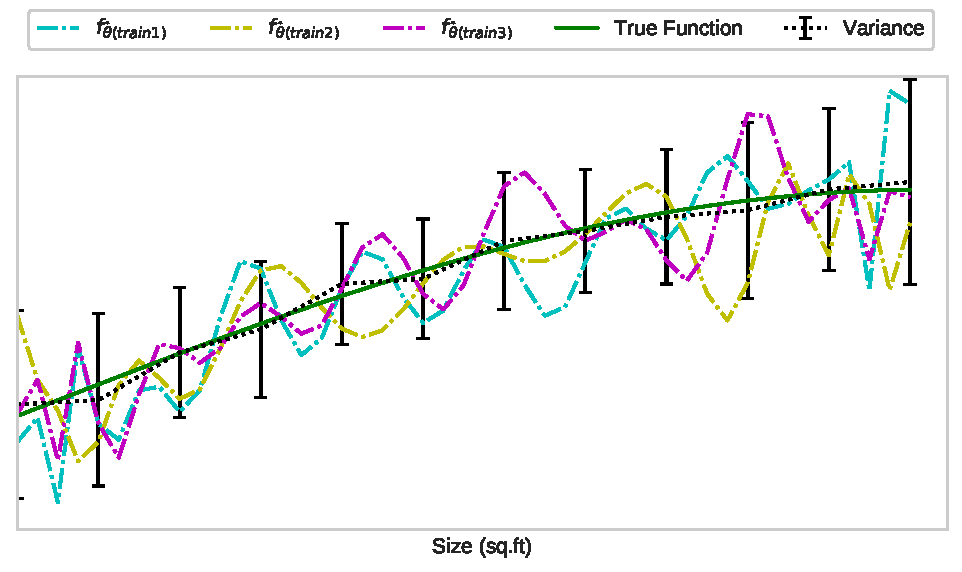
\includegraphics[width=0.8\textwidth]{../assets/bias-variance/figures/var4.pdf}
\vspace*{-0.3cm}
\caption{Variance of a fit}
\end{figure}}
\end{frame}

\begin{frame}{Deriving Expected Prediction Error}
Now we will see how, 
$ E_{train}[\text{at a point } x_t] = \sigma^2 + [\text{bias}(f_{\hat{\theta}}(x_t))]^2 + \text{var}(f_{\hat{\theta}}(x_t)) $

where, 

given a training set, the parameters $\hat{\theta}$ of the fit are learned as $f_{\hat{\theta}}$ 

and, the prediction at a point $x_t$ for the model trained on that training set is $f_{\hat{\theta}}(x_t)$
\end{frame}

\begin{frame}{Deriving Expected Prediction Error}
Prediction Error at a point $x_t$ can be calculated using the squared loss function.\\
\vspace{0.5cm}
 Prediction error at $x_t$ = $(y_t - f_{\hat\theta(train)}(x_t))^2$\\
\vspace{0.5cm}
To find the ``Expected Prediction Error'' at a point $x_t$ we average out the prediction error at that point over all possible learned models. This can be done by finding the expectation of prediction error for that point over all possible training datasets ($train$) and labels for that point ($y_t$).  \\
\vspace{0.5cm}
Expected prediction error at $x_t$ = $E_{train,y_t}[(y_t - f_{\hat\theta(train)}(x_t))^2]$\\
\end{frame}

\begin{frame}{Deriving Expected Prediction Error}
Expected prediction error at $x_t$ = $E_{train,y_t}[(y_t - f_{\hat\theta(train)}(x_t))^2]$\\
\vspace{0.5cm}
\only<2>{
=  $E_{train,y_t}[(          (y_t - f_{\theta(true)}(x_t))     + (f_{\theta(true)}(x_t) -  f_{\hat\theta(train)}(x_t) )            )^2]$
}
\only<3->{
=  $E_{train,y_t}[(      \underbrace{(y_t - f_{\theta(true)}(x_t))}_\text{a}   +   \underbrace{(f_{\theta(true)}(x_t) -  f_{\hat\theta(train)}(x_t) ) }_\text{b}          )^2]$\\
\vspace{0.5cm}
}
\only<4->{
=  $E_{train,y_t}[(a + b) ^ 2]$\\
\vspace{0.5cm}
}
\only<5->{
=  $E_{train,y_t}[a^2 + 2ab + b^2]$\\
\vspace{0.5cm}
}
\only<6->{
(Using Linearity of Expectation)\\
=  $E_{train,y_t}[a^2] + 2E_{train,y_t}[ab] + E_{train,y_t}[b^2]$.......................(Eqn. 1) \\
}

\end{frame}

\begin{frame}{Deriving Expected Prediction Error}
$E_{train,y_t}[a^2]  = E_{train,y_t}[(y_t - f_{\theta(true)}(x_t))^2] $\\
\vspace{0.5cm}
\only<2>{
 \hspace{1.70cm}(Since there is no dependence on training set)\\
\hspace{1.70cm} $ =  E_{y_t}[(y_t - f_{\theta(true)}(x_t))^2] $\\
 \vspace{0.5cm}
}
\only<3->{
 \hspace{1.70cm}($\because$ there is no dependence on training set)\\
 \vspace{0.3cm}
\hspace{1.70cm} $ =  E_{y_t}[\underbrace{(y_t - f_{\theta(true)}(x_t))^2}_\text{$\epsilon_t^2$}] $\\
 \vspace{0.5cm}
}
\only<3->{
\hspace{1.70cm} $ =  E_{y_t}[\epsilon_t^2] $\\
 \vspace{0.5cm}
}
\only<4->{
\hspace{1.70cm} $ =  \sigma^2 $(By definition) \\
 \vspace{0.5cm}
}

\only<5->{
$ E_{train,y_t}[a^2] =  \sigma^2  $.................(Eqn. 2)\\
 \vspace{0.5cm}
}
\end{frame}

\begin{frame}{Deriving Expected Prediction Error}
\only<1>{
$E_{train,y_t}[ab]  = E_{train,y_t}[(y_t - f_{\theta(true)}(x_t))(f_{\theta(true)}(x_t) -  f_{\hat\theta(train)}(x_t) )] $\\
\vspace{0.5cm}
}
\only<2->{
$E_{train,y_t}[ab]  = E_{train,y_t}[\underbrace{(y_t - f_{\theta(true)}(x_t))}_\text{$\epsilon_t$}(f_{\theta(true)}(x_t) -  f_{\hat\theta(train)}(x_t) )] $\\
\vspace{0.5cm}
}
\only<3->{
\hspace{1.70cm} $= E_{train,y_t}[\epsilon_t (f_{\theta(true)}(x_t) -  f_{\hat\theta(train)}(x_t) )] $\\
\vspace{0.5cm}
}
\only<4>{
\hspace{1.70cm} ( $\because \epsilon_t$ and $(f_{\theta(true)}(x_t) -  f_{\hat\theta(train)}(x_t))$ are independent)\\
\vspace{0.3cm}
\hspace{1.70cm} $= E_{train,y_t}[\epsilon_t] \times E_{train,y_t}[(f_{\theta(true)}(x_t) -  f_{\hat\theta(train)}(x_t) )] $\\
\vspace{0.5cm}
}
\only<5->{
\hspace{1.70cm} ( $\because \epsilon_t$ and $(f_{\theta(true)}(x_t) -  f_{\hat\theta(train)}(x_t))$ are independent)\\
\vspace{0.3cm}
\hspace{1.70cm} $= \underbrace{E_{train,y_t}[\epsilon_t]}_\text{ = 0 } \times E_{train,y_t}[(f_{\theta(true)}(x_t) -  f_{\hat\theta(train)}(x_t) )] $\\
\vspace{0.25cm}
\hspace{1.70cm} (By definition $\epsilon_t$ has mean 0)\\
\vspace{0.5cm}
}
\only<6->{
$E_{train,y_t}[ab] = 0$..............(Eqn. 3)
}

\end{frame}

\begin{frame}{Deriving Expected Prediction Error}
$ E_{train,y_t}[b^2] =  E_{train, y_t}[(f_{\theta(true)}(x_t) -  f_{\hat\theta(train)}(x_t) )^2]$\\
\vspace{0.5cm}
\only<2->{
($f_{\theta(true)}(x_t) -  f_{\hat\theta(train)}(x_t)$ is independent of $y_t$)\\
\vspace{0.5cm}
\hspace{1.70cm} $=  E_{train}[(f_{\theta(true)}(x_t) -  f_{\hat\theta(train)}(x_t) )^2]$\\
\vspace{0.5cm}
}
\only<3->{
\hspace{1.70cm} $ = MSE( f_{\hat\theta(train)}(x_t))$\\
\vspace{0.5cm}
}
\only<4->{
$ E_{train,y_t}[b^2] = MSE( f_{\hat\theta(train)}(x_t))$ ............ (Eqn. 4)
}
\end{frame}

\begin{frame}{Deriving Expected Prediction Error}
From Eqn. 1, 2, 3 and 4, we get, \\
\vspace{1cm}
Expected prediction error at $x_t$ = $\sigma^2 + MSE( f_{\hat\theta(train)}(x_t)) $ \\
\vspace{1cm}
Now, we will further simplify the MSE term into bias and variance.
\end{frame}

\begin{frame}{Deriving Expected Prediction Error}
$MSE( f_{\hat\theta(train)}(x_t)) =  E_{train}[(f_{\theta(true)}(x_t) -  f_{\hat\theta(train)}(x_t) )^2]$\\
\vspace{0.5cm}
\only<2>{
$= E_{train}[(   (f_{\theta(true)}(x_t)  -  f_{\bar\theta}(x_t) ) + (f_{\bar\theta}(x_t)  -  f_{\hat\theta(train)}(x_t)      ) )^2]$\\
}
\only<3->{
$= E_{train}[(   \underbrace{(f_{\theta(true)}(x_t)  -  f_{\bar\theta}(x_t) )}_\text{$\alpha$} + \underbrace{(f_{\bar\theta}(x_t)  -  f_{\hat\theta(train)}(x_t)      )}_\text{$\beta$} )^2]$\\
\vspace{0.5cm}
}
\only<4->{
$= E_{train}[( \alpha + \beta )^2]$\\
\vspace{0.5cm}
}
\only<5->{
$= E_{train}[ \alpha^2 + 2\alpha\beta + \beta ^2]$\\
\vspace{0.5cm}
}
\only<6->{
(Using Linearity of Expectation)
$= E_{train}[ \alpha^2] + 2E_{train}[ \alpha\beta] + E_{train}[ \beta^2]$ ..........(Eqn. 5)\\
\vspace{0.5cm}
}
\end{frame}

\begin{frame}{Deriving Expected Prediction Error}
$E_{train}[\alpha^2]  = E_{train}[(f_{\theta(true)}(x_t)  -  f_{\bar\theta}(x_t))^2]$\\
\vspace{0.5cm}
\only<2->{
\hspace{1.45cm} $  = E_{train}[(f_{\theta(true)}(x_t)  -  E_{train}[f_{\hat\theta(train)}(x_t)]^2]$\\
\vspace{0.5cm}
}
\only<3->{
\hspace{1.45cm} $ = E_{train}[bias(f_{\hat\theta}(x_t))^2]$\hfill(By definition of bias)\\
\vspace{0.5cm}
}
\only<4->{
\hspace{1.45cm} $ = bias(f_{\hat\theta}(x_t))^2 $\\
\vspace{0.5cm}
\hspace{1.45cm} ($\because$ bias is not a function of training data)\\

}
\only<5->{
\vspace{0.5cm}
$E_{train}[\alpha^2]  = bias(f_{\hat\theta}(x_t))^2$ .............(Eqn. 6)
}
\end{frame}

\begin{frame}{Deriving Expected Prediction Error}
$E_{train}[\alpha\beta] $ \\
$= E_{train}[(f_{\theta(true)}(x_t)  -  f_{\bar\theta}(x_t))(f_{\bar\theta}(x_t)  -  f_{\hat\theta(train)}(x_t)   )]$\\
\vspace{0.5cm}
\only<2->{
$ = E_{train}[bias_t \times (f_{\bar\theta}(x_t)  -  f_{\hat\theta(train)}(x_t)   )]$\\
\vspace{0.5cm}
}
\only<3->{
$ = bias_t \times E_{train}[f_{\bar\theta}(x_t)  -  f_{\hat\theta(train)}(x_t)  ]$\\
\vspace{0.5cm}
($\because$ bias$_t$ is not a function of training data)\\
\vspace{0.5cm}
}
\only<4->{
$ = bias \times \left( E_{train}[f_{\bar\theta}(x_t)]  -  E_{train}[f_{\hat\theta(train)}(x_t) ] \right)$\\
\vspace{0.5cm}
}
\only<5>{
$ = bias \times \left( f_{\bar\theta}(x_t)  -  f_{\bar\theta}(x_t)  \right) $\\
\vspace{0.5cm}
($\because f_{\bar\theta}(x_t) =  E_{train}[f_{\hat\theta(train)}(x_t)$ )\\
\vspace{0.5cm}
}
\only<6->{
$ = bias \times \left( f_{\bar\theta}(x_t)  -  f_{\bar\theta}(x_t)  \right) $\\
\vspace{0.5cm}
$E_{train}[\alpha\beta]  = 0$..........................(Eqn. 7) 
\vspace{0.5cm}
}

\end{frame}

\begin{frame}{Deriving Expected Prediction Error}
$E_{train}[\beta^2]  = E_{train}[(f_{\bar\theta}(x_t)  -  f_{\hat\theta(train)}(x_t) )^2]$ \\
\vspace{0.5cm}
\only<2->{
\hspace{1.45cm} $=  E_{train}[(f_{\hat\theta(train)}(x_t) - f_{\bar\theta}(x_t))^2]$\\
\vspace{0.5cm}
}
\only<3->{
\hspace{1.45cm} $=  E_{train}[(f_{\hat\theta(train)}(x_t) - E_{train}[(f_{\hat\theta(train)}(x_t)])^2]$\\
\vspace{0.5cm}
\hspace{1.45cm} ($\because f_{\bar\theta}(x_t) = E_{train}[(f_{\hat\theta(train)}(x_t)] $ )\\
\vspace{0.5cm}
}
\only<4->{
\hspace{1.45cm} $= variance(f_{\hat\theta}(x_t))$\\
\vspace{0.5cm}
}
\only<5->{
$E_{train}[\beta^2] = variance(f_{\hat\theta}(x_t))$...............(Eqn. 8)\\
}

\end{frame}

\begin{frame}{Deriving Expected Prediction Error}
From Eqn. 1 - 8, we get, \\
\vspace{0.5cm}
Expected prediction error at $x_t$ \\
\vspace{0.5cm}
$ = \sigma^2 + MSE( f_{\hat\theta(train)}(x_t)) $\\
\vspace{0.5cm}
$ = \sigma^2 +bias(f_{\hat\theta}(x_t))^2 + variance(f_{\hat\theta}(x_t))$

\end{frame}

\end{document}
